\documentclass[11pt,a4paper]{article}
\usepackage[utf8]{inputenc}
\usepackage[margin=0.85in]{geometry}
\usepackage{graphicx}
\usepackage{hyperref}
\usepackage{booktabs}
\usepackage{caption}
\usepackage{float}
\usepackage{enumitem}

\hypersetup{
    colorlinks=true,
    linkcolor=blue,
    filecolor=magenta,      
    urlcolor=cyan,
    pdftitle={Design Document using SA/SD Methodology: Website Vulnerability Scanner},
    pdfpagemode=UseOutlines,
}

\title{\textbf{Design Document using SA/SD Methodology}\\ \Large for\\ \textbf{Website Vulnerability Scanner}}
\author{%
  \textbf{Prepared by}\\[0.5em]
  Deepthi K (241IT021)\\
  Jasmine (241IT051)\\
  Sacheth Koushal (241IT058)\\[1.2em]
  \textbf{Department of Information Technology}\\
  \textbf{National Institute of Technology Karnataka, Surathkal}
}
\date{August 2026}

\begin{document}

\maketitle

\tableofcontents
\newpage

\section{Data Flow Diagram (DFD) Model}

\subsection{Level 0 DFD}
\subsubsection{Context Diagram}

Figure \ref{fig:level0} illustrates the Level 0 Context Diagram for the Website Vulnerability Scanner system. It defines the primary system boundary for Process 0 and models all inbound/outbound interaction channels with key external entities including the WVS User, System Administrator, Target Website, Public DNS Resolvers, SMTP Relay, and OSV/EPSS Advisory APIs.

\begin{figure}[H]
    \centering
    
\includegraphics[width=0.88\textwidth,height=0.48\textheight,keepaspectratio]{mermaid/png/level-0.png}
    \caption{Level 0 Context Diagram}
    \label{fig:level0}
\end{figure}

\subsection{Level 1 DFD}
\subsubsection{Top-Level Functional Decomposition}

Figure \ref{fig:level1} depicts the Level 1 DFD, decomposing Process 0 into 8 primary functional modules ($0.1$ through $0.8$). It displays the primary scanning pipeline from initial user request through scope validation, discovery crawling, vulnerability detection, findings management, and report generation, alongside centralized Scope Guard enforcement ($0.8$) and third-party integrations.

\begin{figure}[H]
    \centering
    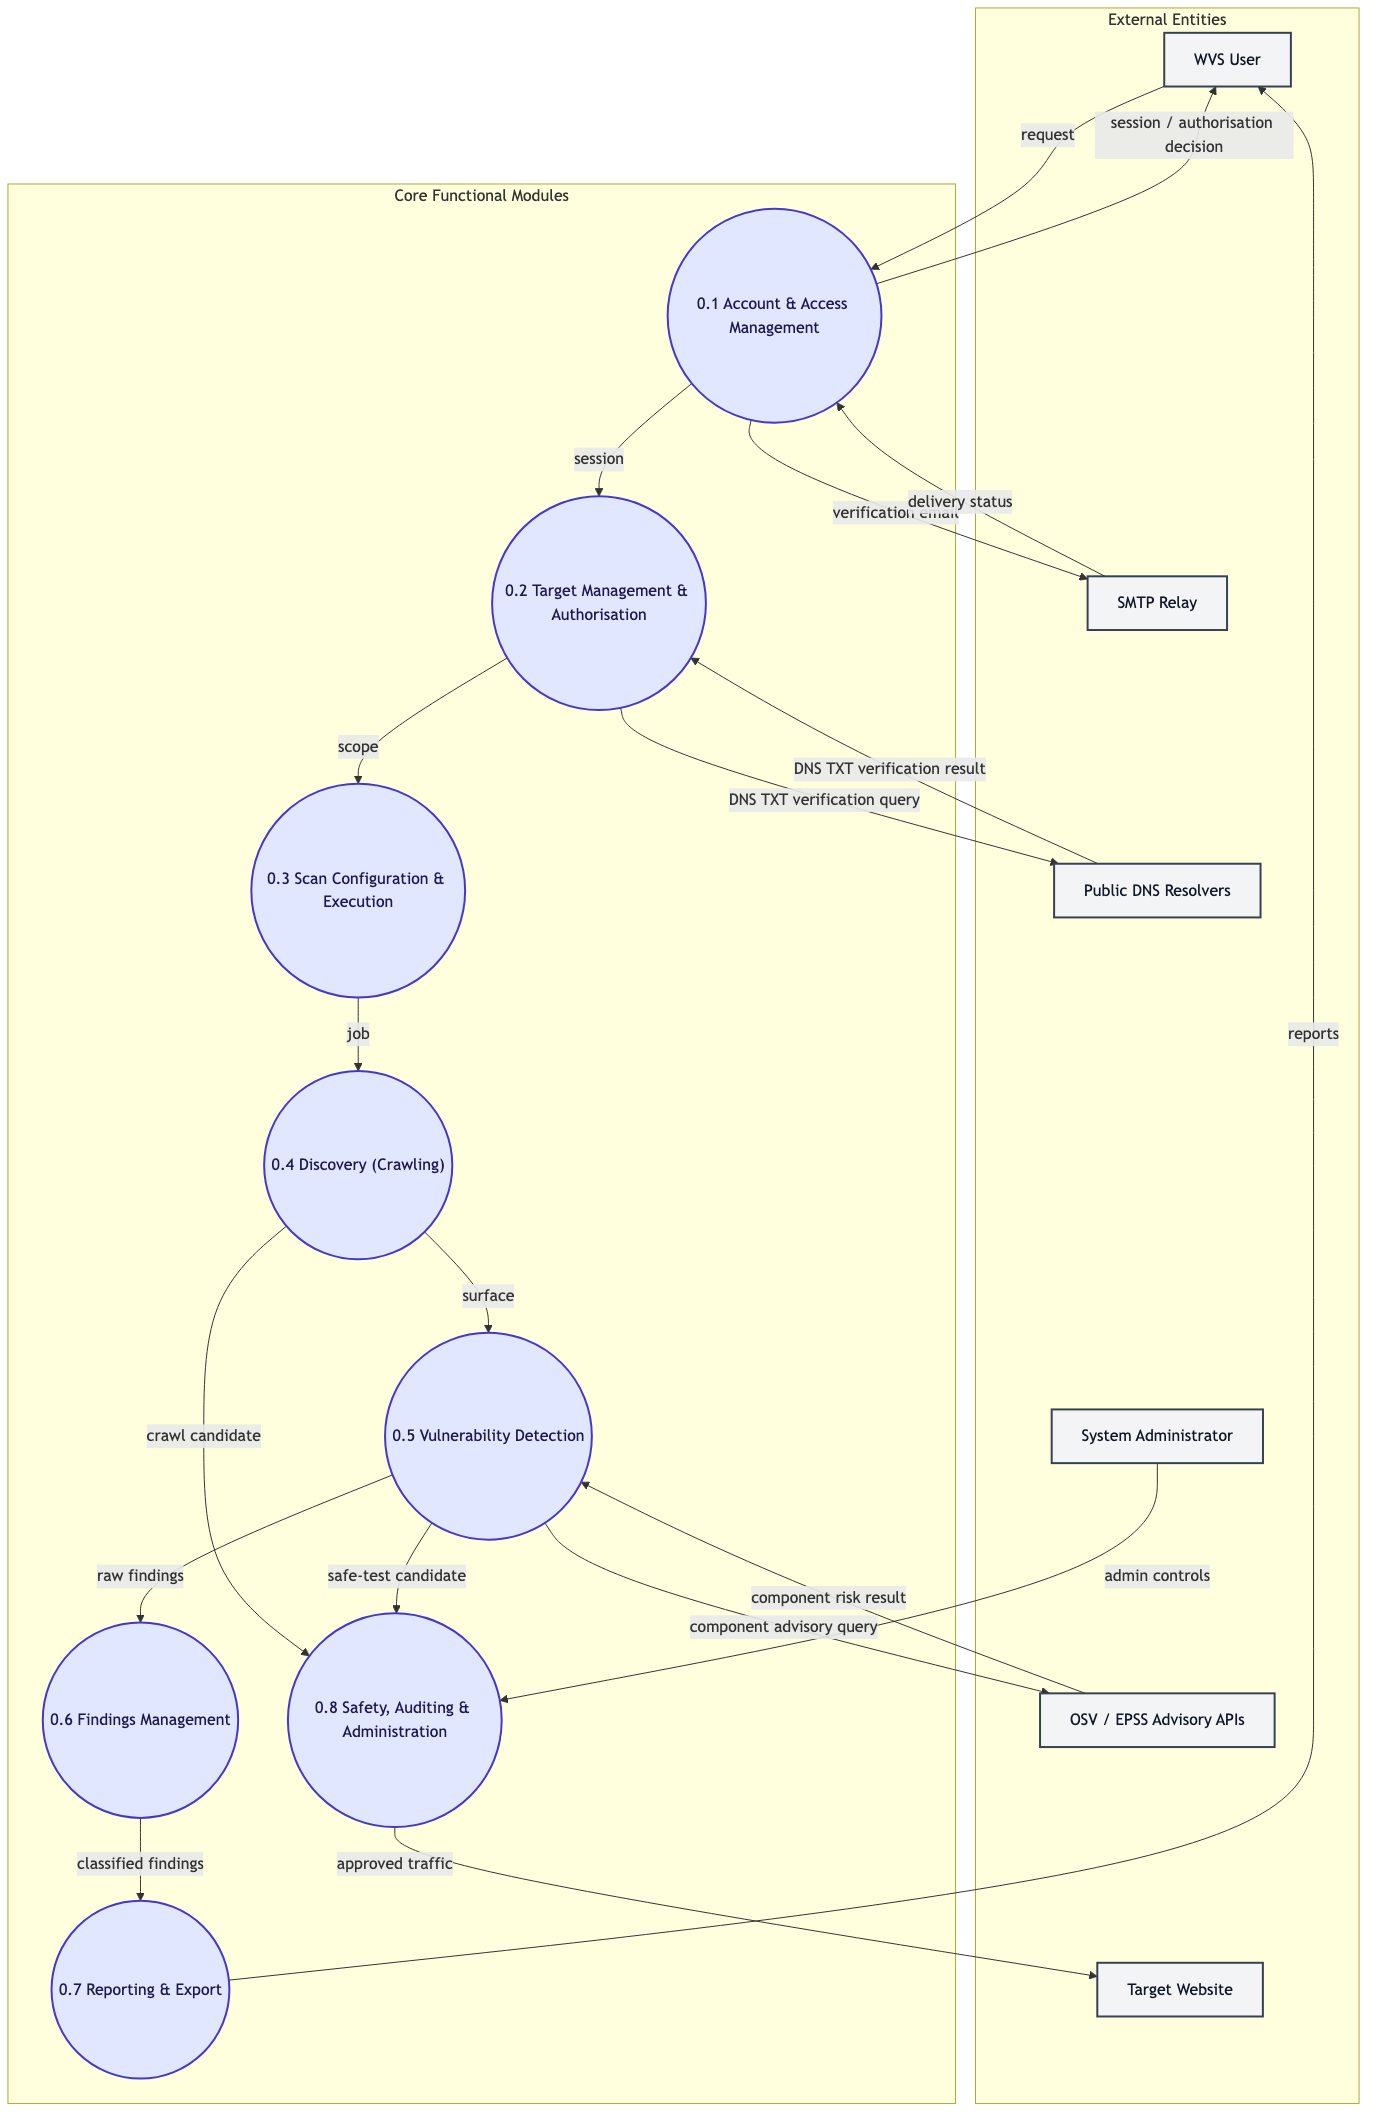
\includegraphics[width=0.94\textwidth,height=0.85\textheight,keepaspectratio]{mermaid/png/level-1.png}
    \caption{Level 1 DFD with 8 functional groups}
    \label{fig:level1}
\end{figure}

\newpage
\subsection{Level 2 DFDs}

\subsubsection{0.1 User Authentication \& Access Control}

Decomposes Process $0.1$ into credential validation, session token issuance, and login audit logging. Process 1.1 validates user credentials against Data Store D1, Process 1.2 issues session tokens and verifies email deliverability via SMTP Relay, and Process 1.3 records authentication audits.

\begin{figure}[H]
    \centering
    
\includegraphics[width=0.94\textwidth,height=0.75\textheight,keepaspectratio]{mermaid/png/f.1.png}
    \caption{Level 2 DFD for 0.1 User Authentication \& Access Control}
    \label{fig:f1}
\end{figure}

\subsubsection{0.2 Target Management \& Authorisation}

Decomposes Process $0.2$ into target registration, verification token generation, and DNS/well-known proof validation. Process 2.1 registers target definitions in D2, Process 2.2 generates ownership tokens verified against Public DNS, and Process 2.3 checks well-known path tokens on the Target Website.

\begin{figure}[H]
    \centering
    
\includegraphics[width=0.94\textwidth,height=0.75\textheight,keepaspectratio]{mermaid/png/f.2.png}
    \caption{Level 2 DFD for 0.2 Target Management \& Authorisation}
    \label{fig:f2}
\end{figure}

\newpage
\subsubsection{0.3 Scan Configuration \& Execution}

Decomposes Process $0.3$ into scan profile validation, job scheduling, and lifecycle execution. Process 3.1 verifies user scope and quotas against D2, Process 3.2 queues scan jobs in D3, and Process 3.3 executes the scan lifecycle while writing reproducibility records to D4.

\begin{figure}[H]
    \centering
    
\includegraphics[width=0.94\textwidth,height=0.75\textheight,keepaspectratio]{mermaid/png/f.3.png}
    \caption{Level 2 DFD for 0.3 Scan Configuration \& Execution}
    \label{fig:f3}
\end{figure}

\subsubsection{0.4 Discovery (Crawling)}

Decomposes Process $0.4$ into scope loading, link/form discovery, and JS rendering deduplication. Process 4.1 loads ceilings from D2, Process 4.2 dispatches crawl candidates to Process 0.8 Scope Guard, and Process 4.3 records page inventory in D4 upon receiving HTTP responses from the Target Website.

\begin{figure}[H]
    \centering
    
\includegraphics[width=0.94\textwidth,height=0.75\textheight,keepaspectratio]{mermaid/png/f.4.png}
    \caption{Level 2 DFD for 0.4 Discovery (Crawling)}
    \label{fig:f4}
\end{figure}

\newpage
\subsubsection{0.5 Vulnerability Detection}

Decomposes Process $0.5$ into passive header checking, safe active test preparation, and advisory version enrichment. Process 5.1 runs passive analysis, Process 5.2 routes active test payloads through Process 0.8 Scope Guard, and Process 5.3 queries OSV/EPSS APIs and stores evidence in D5.

\begin{figure}[H]
    \centering
    
\includegraphics[width=0.94\textwidth,height=0.75\textheight,keepaspectratio]{mermaid/png/f.5.png}
    \caption{Level 2 DFD for 0.5 Vulnerability Detection}
    \label{fig:f5}
\end{figure}

\subsubsection{0.6 Findings Management}

Decomposes Process $0.6$ into normalisation/redaction, historical scan comparison, and triage filtering. Process 6.1 ingests raw findings, Process 6.2 compares historical evidence stored in D5, and Process 6.3 applies user triage filters and severity classification.

\begin{figure}[H]
    \centering
    
\includegraphics[width=0.94\textwidth,height=0.75\textheight,keepaspectratio]{mermaid/png/f.6.png}
    \caption{Level 2 DFD for 0.6 Findings Management}
    \label{fig:f6}
\end{figure}

\newpage
\subsubsection{0.7 Reporting \& Export}

Decomposes Process $0.7$ into completed scan selection, report template assembly, and export dispatch. Process 7.1 retrieves scan metadata from D4, Process 7.2 compiles finding evidence from D5, and Process 7.3 generates export files (PDF/CSV) and triggers SMTP notifications.

\begin{figure}[H]
    \centering
    
\includegraphics[width=0.94\textwidth,height=0.75\textheight,keepaspectratio]{mermaid/png/f.7.png}
    \caption{Level 2 DFD for 0.7 Reporting \& Export}
    \label{fig:f7}
\end{figure}

\subsubsection{0.8 Safety, Auditing \& Administration}

Decomposes Process $0.8$ into scope/blocklist verification, IP re-resolution \& rate limiting, and request dispatch. Process 8.1 evaluates requests against D2 policies, Process 8.2 performs fresh DNS checks to prevent SSRF, and Process 8.3 logs dispatches to D6 Append-only Audit Ledger.

\begin{figure}[H]
    \centering
    
\includegraphics[width=0.94\textwidth,height=0.75\textheight,keepaspectratio]{mermaid/png/f.8.png}
    \caption{Level 2 DFD for 0.8 Safety, Auditing \& Administration}
    \label{fig:f8}
\end{figure}

\newpage
\section{Core Modules}

This section describes the core functional modules of the Website Vulnerability Scanner. Each module manages a distinct phase of the scanning lifecycle.

\subsection{0.1 User Authentication \& Access Control}
Handles user authentication, organisation onboarding, session management, and multi-factor verification.
\begin{itemize}[noitemsep]
    \item \textbf{Functions}: Register User, Validate Credentials \& MFA, Issue Session Token (JWT), Audit Login \& Enforce Lockout.
\end{itemize}

\subsection{0.2 Target Management \& Authorisation}
Manages domain registration, scope definitions, ownership verification tokens, and DNS/well-known target validation.
\begin{itemize}[noitemsep]
    \item \textbf{Functions}: Register Target \& Scope, Issue Verification Token, Validate DNS TXT / Well-Known Proof, Store Scope Rules.
\end{itemize}

\subsection{0.3 Scan Configuration \& Execution}
Validates scan profile settings, checks user quotas, queues execution jobs, and manages lifecycle execution checkpoints.
\begin{itemize}[noitemsep]
    \item \textbf{Functions}: Validate Profile \& Quota, Queue Scan Job / Schedule, Execute Lifecycle \& Checkpoint, Record Scan Reproducibility.
\end{itemize}

\subsection{0.4 Discovery (Crawling)}
Extracts attack surface elements including links, forms, API endpoints, and dynamic JS content while abiding by crawl ceilings.
\begin{itemize}[noitemsep]
    \item \textbf{Functions}: Load Scope \& Ceilings, Discover Links \& Sitemap, Render JS \& Deduplicate, Dispatch Candidates to Scope Guard.
\end{itemize}

\subsection{0.5 Vulnerability Detection}
Performs non-destructive vulnerability checks, passive header analysis, active payload testing via Scope Guard, and advisory database lookup.
\begin{itemize}[noitemsep]
    \item \textbf{Functions}: Run Passive Response Checks, Prepare Safe Active Checks, Enrich Component Versions via OSV/EPSS APIs.
\end{itemize}

\subsection{0.6 Findings Management}
Normalises raw scan evidence, redacts sensitive tokens, correlates findings against prior scan runs, and applies triage filters.
\begin{itemize}[noitemsep]
    \item \textbf{Functions}: Normalise \& Redact Findings, Compare Prior Scan Evidence, Apply Triage, Filtering \& Severity Sorting.
\end{itemize}

\subsection{0.7 Reporting \& Export}
Assembles executive and technical report documents, formats exports (PDF/CSV), and dispatches completion notifications.
\begin{itemize}[noitemsep]
    \item \textbf{Functions}: Select Completed Scan, Assemble Report Template \& Evidence, Generate Export / Share Link, Send SMTP Notification.
\end{itemize}

\subsection{0.8 Safety, Auditing \& Administration}
Enforces safety invariants, validates target scope, re-resolves DNS to prevent TOCTOU/SSRF attacks, applies rate limits, and maintains an append-only URL ledger.
\begin{itemize}[noitemsep]
    \item \textbf{Functions}: Check Verification \& Scope Blocklist, Re-resolve IP \& Rate-Limit, Dispatch Approved Request, Append Audit Log.
\end{itemize}

\section{Structure Charts}

\subsection{Level 1 Structure Chart}
\subsubsection{Module Decomposition}

The system module hierarchy follows a structured top-down functional decomposition, decoupling user interface and management services from the core crawling engine, detection modules, and centralized Scope Guard safety layer. Figure \ref{fig:structure_chart} illustrates the Level 1 Structure Chart of the System.

\begin{figure}[H]
    \centering
    
\includegraphics[width=0.95\textwidth,height=0.42\textheight,keepaspectratio]{mermaid/png/structure-chart.png}
    \caption{Level 1 Structure Chart of the System}
    \label{fig:structure_chart}
\end{figure}

\end{document}
